\chapter{Tests}


\section{Pictures}


% example for the protocol chapter... instead of the tables....

\subsection{Protocol boxes}

A bit cumbersome and we would need to have text at defined locations. Perhaps keep the simple table in the protocol chapter.

\begin{center}
\begin{tikzpicture}[scale=0.9, transform shape]

    \draw[help lines, gray!50, dashed] (0,0) grid( 16,8);

    \node[  draw, 
            tsRoundedRectangle, 
            minimum width=6cm, 
            minimum height=4cm, 
            text height=1cm, 
            align=left] (A) at (4, 4) 
            { };

    \node[  draw, 
            tsRoundedRectangle, 
            minimum width=6cm, 
            minimum height=4cm, 
            text height=1cm, 
            align=left] (B) at (12, 4) 
            { };

    \draw[->] (A.north east) ++(0, -1) -- ($(B.west) + (0, 1 )$);
    \draw[->] (B.south west) ++(0,  1) -- ($(A.east) + (0, -1)$);

    \node at ( 4,  6.25 ) {\textbf{Node A}};
    \node at ( 12, 6.25 ) {\textbf{Node B}};

    \node at ( 2.25,  5 ) {\textbf{LCS\_TOF}};
    \node at ( 10.25, 3 ) {\textbf{LCS\_TOF}};

\end{tikzpicture}
\end{center}




\subsection{Instruction Word Layout}

We would need an instruction word layout... just a test...

\begin{center}
    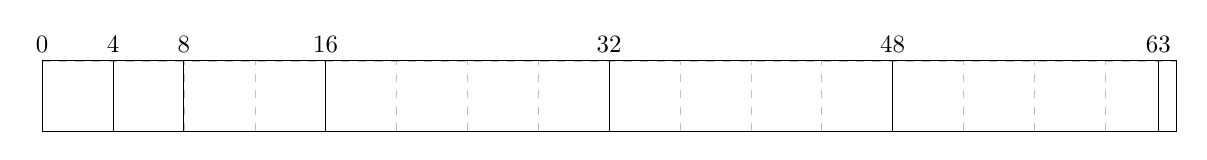
\begin{tikzpicture}[scale=0.9, transform shape]
    
    	\draw[help lines, gray!50, dashed] (0,0) grid(16,1);
    
        % Box for the 64-bit instruction word
        \draw (0,0) rectangle (16,1);

	
         % Bit separators (adjust positions as needed)
        \foreach \x/\label in {0/0, 4/4, 8/8, 16/16, 32/32, 48/48, 63/63} {
            \draw (\x/64*16, 0) -- (\x/64*16, 1); % Scale bit position to 16 cm width
            \node[above] at (\x/64*16, 1) {\label}; % Bit position labels
        }

    \end{tikzpicture}
\end{center}




